
%(BEGIN_QUESTION)
% Copyright 2014, Tony R. Kuphaldt, released under the Creative Commons Attribution License (v 1.0)
% This means you may do almost anything with this work of mine, so long as you give me proper credit

Determine all component voltages and currents in this circuit, being sure to mark directions of all currents (conventional flow notation) and polarities of all voltages:

$$\includegraphics[width=15.5cm]{i02272x01.eps}$$

Also, identify the amount of voltage between points A and B.

\vfil 

\underbar{file i02272}
\eject
%(END_QUESTION)





%(BEGIN_ANSWER)

This is a graded question -- no answers or hints given!

%(END_ANSWER)





%(BEGIN_NOTES)

$$I_{7k3} = {5.5 \hbox{ V} \over 7300 \> \Omega} =  0.753 \hbox{ mA}$$

Voltage across the series resistor pair (same as voltage across the 10k resistor) will be equal to this amount of current times the resistance of the series pair:

$$V_{10k} = (0.753 \hbox{ mA}) (8800 \> \Omega) = 6.630 \hbox{ V}$$

Current through the 10k resistor is simply the quotient of this voltage drop and 10000 ohms:

$$I_{10k} = {6.630 \hbox{ V} \over 10000 \> \Omega} = 0.663 \hbox{ mA}$$

Total current (same as current through the 3300 ohm resistor) will be the sum of these two currents:

$$I_{total} = 0.753 \hbox{ mA} + 0.663 \hbox{ mA} = 1.416 \hbox{ mA}$$

Finding voltage between points A and B is possible by adding the voltage drops of the 7.3k ohm resistor and the 3.3k ohm resistor:

$$V_{AB} = 5.5 \hbox{ V} + I_{total} (3300 \> \Omega)$$

$$V_{AB} = 5.5 \hbox{ V} + (1.416 \hbox{ mA}) (3300 \> \Omega)$$

$$V_{AB} = 5.5 \hbox{ V} + 4.674 \hbox{ V}$$

$$V_{AB} = 10.17 \hbox{ V, with A positive and B negative}$$

$$\includegraphics[width=15.5cm]{i02272x02.eps}$$

%INDEX% Electronics review: Kirchhoff's Voltage Law (KVL)

%(END_NOTES)


